\chapter{Programátorská dokumentace}
V této kapitole popíšeme naší implementaci platformy MHUrho a ukázkové hry. K implementaci platformy bylo použito Visual Studio 2017 Education a .NET Framework 4.7.2, který je zároveň cílovým frameworkem naší platformy. Celá implementace je obsažena v jediném \uv{solution}, MHUrho. 

\section{Struktura solution}

\begin{figure}[h]
	\centering
	\fontsize{10pt}{11pt}\selectfont
	\def\svgwidth{0.9\textwidth}
	\input{img/Project_structure.pdf_tex}
	\caption{Struktura solution. Zelené značí součásti naší práce, oranžové místo budoucí rozšiřitelnosti.}
	\label{fig:solution_structure}
\end{figure}

Hlavním cílem naší práce byla tvorba platformy pro tvorbu RTS her. Jak můžeme vidět v diagramu \ref{fig:solution_structure}, vlastní implementace platformy je realizována několika projekty. Účelem tohoto rozdělení je separace přenositelně implementovatelných částí platformy, které díky využití enginu UrhoSharp a celkovému návrhu práce tvoří velkou většinu funkcionality, od částí závislých na cílovém systému. 

Přenositelné části jsou obsaženy v projektu \texttt{MHUrho}. Výstupem tohoto projektu je knihovna, využívaná jak implementacemi pro specifické systémy, tak balíčky tvořícími jednotlivé hry. 

Implementace pro specifické systémy obsahují především inicializační kód, který dostává spuštěný program do konzistentního stavu bez ohledu na platformu, a dále implementace rozhraní specifikovaných v přenositelné části, které umožňují této části pracovat s oblastmi, pro které ani platforma .NET ani používaný herní engine neposkytují přenositelnou implementaci. Tyto oblasti byli popsány v části \ref{sec:system_dif}.

Dále schéma ukazuje dvě součásti solution, které nejsou přímo součástí funkcionality platformy. První z těchto součástí je projekt \texttt{ShowcasePackage}, který obsahuje implementaci ukázkové hry sloužící pro demonstraci schopností platformy a jako referenční implementace pro tvůrce budoucích balíčku. Druhou součástí je \texttt{Installer}, jehož výstupem je \texttt{.msi} instalátor umožňující jednoduchou instalaci platformy na systém Windows spolu s instalací všech závislostí a vložení \textit{Ukázkového balíčku} do nainstalované instance platformy.

\section{Spuštění aplikace}
\label{sec:init}
Spuštění aplikace je specifické pro každý ze systémů. Vzhledem k tomu, že cílem naší práce byla implementace platformy pro systém Windows, popíšeme v této části spuštění aplikace v rámci tohoto systému.

\subsection{Systémová část}

\begin{figure}[h]
	\centering
	\fontsize{8pt}{11pt}\selectfont
	\def\svgwidth{\textwidth}
	\input{img/MHUrhoApp2.pdf_tex}
	\caption{Spouštění aplikace.}
	\label{fig:startup}
\end{figure}

Spuštění začíná v implementaci specifické pro daný systém. Hlavní třídy účastnící se spuštění aplikace a posloupnost volání metod můžeme vidět na obrázku \ref{fig:startup}. U každé ze tříd jsou ilustrovány pouze prvky účastnící se inicializace. 

Pro systém Windows začíná celý proces jako ve většině aplikací zavoláním metody \texttt{Main}. Tato metoda jako první inicializuje \texttt{FileManager}, implementující práci se soubory na systému Windows, a uloží ho do statické položky třídy \texttt{MHUrhoApp}. Tento systém je nezbytné inicializovat před spuštěním herního enginu, protože je používán při inicializaci třídy \texttt{MHUrhoApp}.

Jak ukazuje diagram, třída \texttt{MHUrhoApp} je potomkem třídy \texttt{Application} z namespace \texttt{Urho}. Tato třída, již podle názvu, reprezentuje celou aplikaci v enginu UrhoSharp a poskytuje přístup ke všem ostatním součástem enginu. 

Dalším krokem v metodě \texttt{Main} je zpracování parametrů aplikace z příkazového řádku do systémově nezávislé reprezentace. Tato reprezentace je následně také uložena do statické položky třídy \texttt{MHUrhoApp}, protože je stejně jako \texttt{FileManager} používána při inicializaci MHUrhoApp.

Položky \texttt{FileManager} a \texttt{StartupArgs} jsou statické pro budoucí rozšiřitelnost na platformu Android.
Důvodem je nutnost spuštění enginu pomocí následujícího kódu:

\begin{lstlisting}
await surface.Show<MHUrhoApp>(new ApplicationOptions("Data"));
\end{lstlisting}

Metoda \texttt{Show} bohužel nedovoluje přidat konstruktoru \texttt{MHUrhoApp} další parametry, kterými by bylo možné předat \texttt{FileManager} a \texttt{StartupOptions}.

Na systému Windows následuje vytvoření instance \texttt{MHUrhoApp} a zavolání metody \texttt{Run}. Tímto voláním se předává kontrola enginu UrhoSharp, který je tímto inicializován a je v něm spuštěna herní smyčka.

V rámci své inicializace zavolá herní engine virtuální metodu \texttt{Start}, jejíž přetížením nám umožňuje inicializovat si naší část aplikace. Tímto se dostáváme do přenositelné části inicializace.

\subsection{Přenositelná část}

Jak je řečeno v předchozí části, přenositelná část inicializace začíná v okamžiku volání metody \texttt{Start} herním enginem.

V rámci této metody provede platforma inicializaci všech svých součástí a přejde do režimu reagování na interakce uživatele s grafickým rozhraním.


\section{Uživatelské rozhraní}

\begin{figure}[h]
	\centering
	\fontsize{8pt}{11pt}\selectfont
	\def\svgwidth{\textwidth}
	\input{img/UIReferences.pdf_tex}
	\caption{Datová struktura uživatelského rozhraní.}
	\label{fig:uireferences}
\end{figure}

Jak můžeme vidět na diagramu \ref{fig:uireferences}, centrálními třídami uživatelského rozhraní v rámci menu jsou třídy \texttt{MenuController} a \texttt{MenuUIManager}. Dále můžeme vidět, že z pohledu herního enginu je grafické rozhraní reprezentováno třídou \texttt{UI} s kořenovým prvkem \texttt{Root}.

Účelem třídy \texttt{MenuController} je odstínění implementace uživatelského rozhraní od detailů implementace zbytku platformy. Pokud je tedy výsledkem uživatelovi akce změna stavu jiné části platformy než UI, je tato akce delegována právě třídě \texttt{MenuController}. Zároveň se také tato třída snaží odstiňovat zbytek platformy od implementace uživatelského rozhraní, tedy pokud část hry požaduje změnu uživatelského rozhraní, měla by tuto akci delegovat třídě \texttt{MenuController}.

Třída \texttt{MenuUIManager} je, jak můžeme vidět, centrálním bodem implementace uživatelského rozhraní menu. Její hlavní funkcí je management a poskytnutí přístupu ke všem obrazovkám menu a implementace přepínání mezi obrazovkami. V rámci přepínání obrazovek umožňuje tato třída jednoduše přepínat zpět na předchozí obrazovky, protože při každém přepnutí na novou obrazovku je tato obrazovka přidána do zásobníku předchozích obrazovek.

Každá z obrazovek menu je reprezentována samostatnou třídou, implementující chování obrazovky a zajišťující správu prostředků herního enginu příslušících dané obrazovce. Jak můžeme vidět na diagramu \ref{fig:uireferences}, slouží každá ze tříd reprezentujících obrazovky menu jako \textit{proxy} pro třídu, která implementuje vlastní chování obrazovky a vlastní prostředky enginu pro její zobrazení uživateli. 

Z pohledu enginu tvoří uživatelské rozhraní strom s kořenem \texttt{Root}. Každá obrazovka je tedy dítětem tohoto kořenu, s dalšími prvky jako tlačítky a popisky jako svými dětmi. Tyto prostředky, reprezentující danou obrazovku, jsou zpravovány právě implementační třídou a mají stejnou životnost jako tato třída.

Zobrazení obrazovky je uskutečněno v reakci na zavolání metody \texttt{Show} na \textit{proxy} třídě obrazovky. Metoda \texttt{Show} vytvoří novou instanci implementační třídy, která v rámci konstruktoru použije engine a \texttt{UI.Root} pro nahrání obrazovky. Při následném skrytí obrazovky v reakci na volání metody \texttt{Hide} na proxy třídě je implementační třída zahozena pomocí volání \texttt{Dispose} a nastavení reference na null. V rámci volání \texttt{Dispose} jsou z reprezentace uživatelského rozhraní uvnitře enginu odstraněny všechny prvky příslušící této obrazovce.Díky této implementaci nedochází k hromadění naalokovaných obrazovek i při cyklickém přepínání mezi několika obrazovkami.



\subsection{Definice vzhledu}
Engine UrhoSharp umožňuje definici rozložení a vzhledu uživatelského rozhraní jak v kódu, tak pomocí XML souborů. Podle složitosti jednotlivých obrazovek používáme kombinaci obou těchto možností. Některé jednodušší obrazovky, jako například hlavní menu, mají celý svůj vzhled definovaný pomocí XML souborů. Složitější obrazovky, měnící svůj vzhled v reakci na uživatelské akce, mají základní vzhled definován pomocí XML a následně měněn v kódu dané obrazovky. 

\noindent{Použité XML soubory se rozdělují na dva druhy:}
\begin{enumerate}
	\item definující vzhled,
	\item definující rozložení.
\end{enumerate}

Soubory definující uživatelské rozhraní platformy pro systém Windows jsou uloženy v adresáři \texttt{MHUrho.Desktop/Data/UI/}.
Vzhled prvků rozhraní je definován především v souboru \texttt{MainMenuStyle.xml}, spolu s několika menšími soubory pojmenovanými \uv{\texttt{...Style.xml}}, definujícími vzhled dynamicky přidávaných prvků. Hlavní styl uživatelského rozhraní \texttt{MainMenuStyle.xml} je nastaven v kořeni \texttt{UI.Root} jako defaultní, je tedy aplikován na všechny prvky v celém uživatelském rozhraní pokud jim není přiřazen explicitně jiný vzhled.

Rozložení prvků je pro každou obrazovku v separátním souboru, pojmenovaném \texttt{[Jméno obrazovky]Layout.xml}. Tyto soubory byli vytvořeny za použití editoru enginu Urho3D, který je distribuován spolu s enginem UrhoSharp. 

\subsection{Přepínání obrazovek}
Přepínání obrazovek je jedním z hlavních úkolů třídy \texttt{MenuUIManager}. Tato třída poskytuje metody pro přepnutí na každou z obrazovek. Každá z těchto metod deklaruje data potřebná pro zobrazení dané obrazovky, která následně poskytne třídě reprezentující danou obrazovku.

Posloupnost možných přechodů obrazovek můžeme vidět na diagramu \ref{fig:screen_structure}. Při spuštění aplikace je počáteční obrazovkou hlavní menu. Jak můžeme vidět, z tohoto menu se lze dostat na obrazovky \textit{Package picking}, \textit{Load game}, \textit{Options} a \textit{About}. Dále lze z tohoto menu ukončit celou aplikaci. Každý z černých přechodů přidává starou obrazovku na zásobník obrazovek a nastavuje novou obrazovku jako \texttt{CurrentScreen}, tedy aktuální obrazovku. Tímto způsobem poskytuje třída \texttt{MenuUIManager} možnost tlačítka zpět, které je schopno vracet se v protisměru černých šipek.

Červené šipky v diagramu značí přechod do hry, tedy vyčištění zásobníku obrazovek a zahození aktuální obrazovky. Tímto je uvolněna veškerá nepotřebná paměť zabraná uživatelským rozhraním menu a je přenechána pro běh hry.

Dále můžeme vidět přerušované šipky, které značí přechody bez možnosti návratu touto cestou. Při pozastavení úrovně je hra převedena do obrazovky \textit{Pauza}. Tato obrazovka se mírně liší podle toho, zda jsme se dostali do ní dostali z editované úrovně či z hrané úrovně. Tento rozdíl je implementován podle návrhového vzoru Strategy.

\begin{figure}[h]
	\centering
	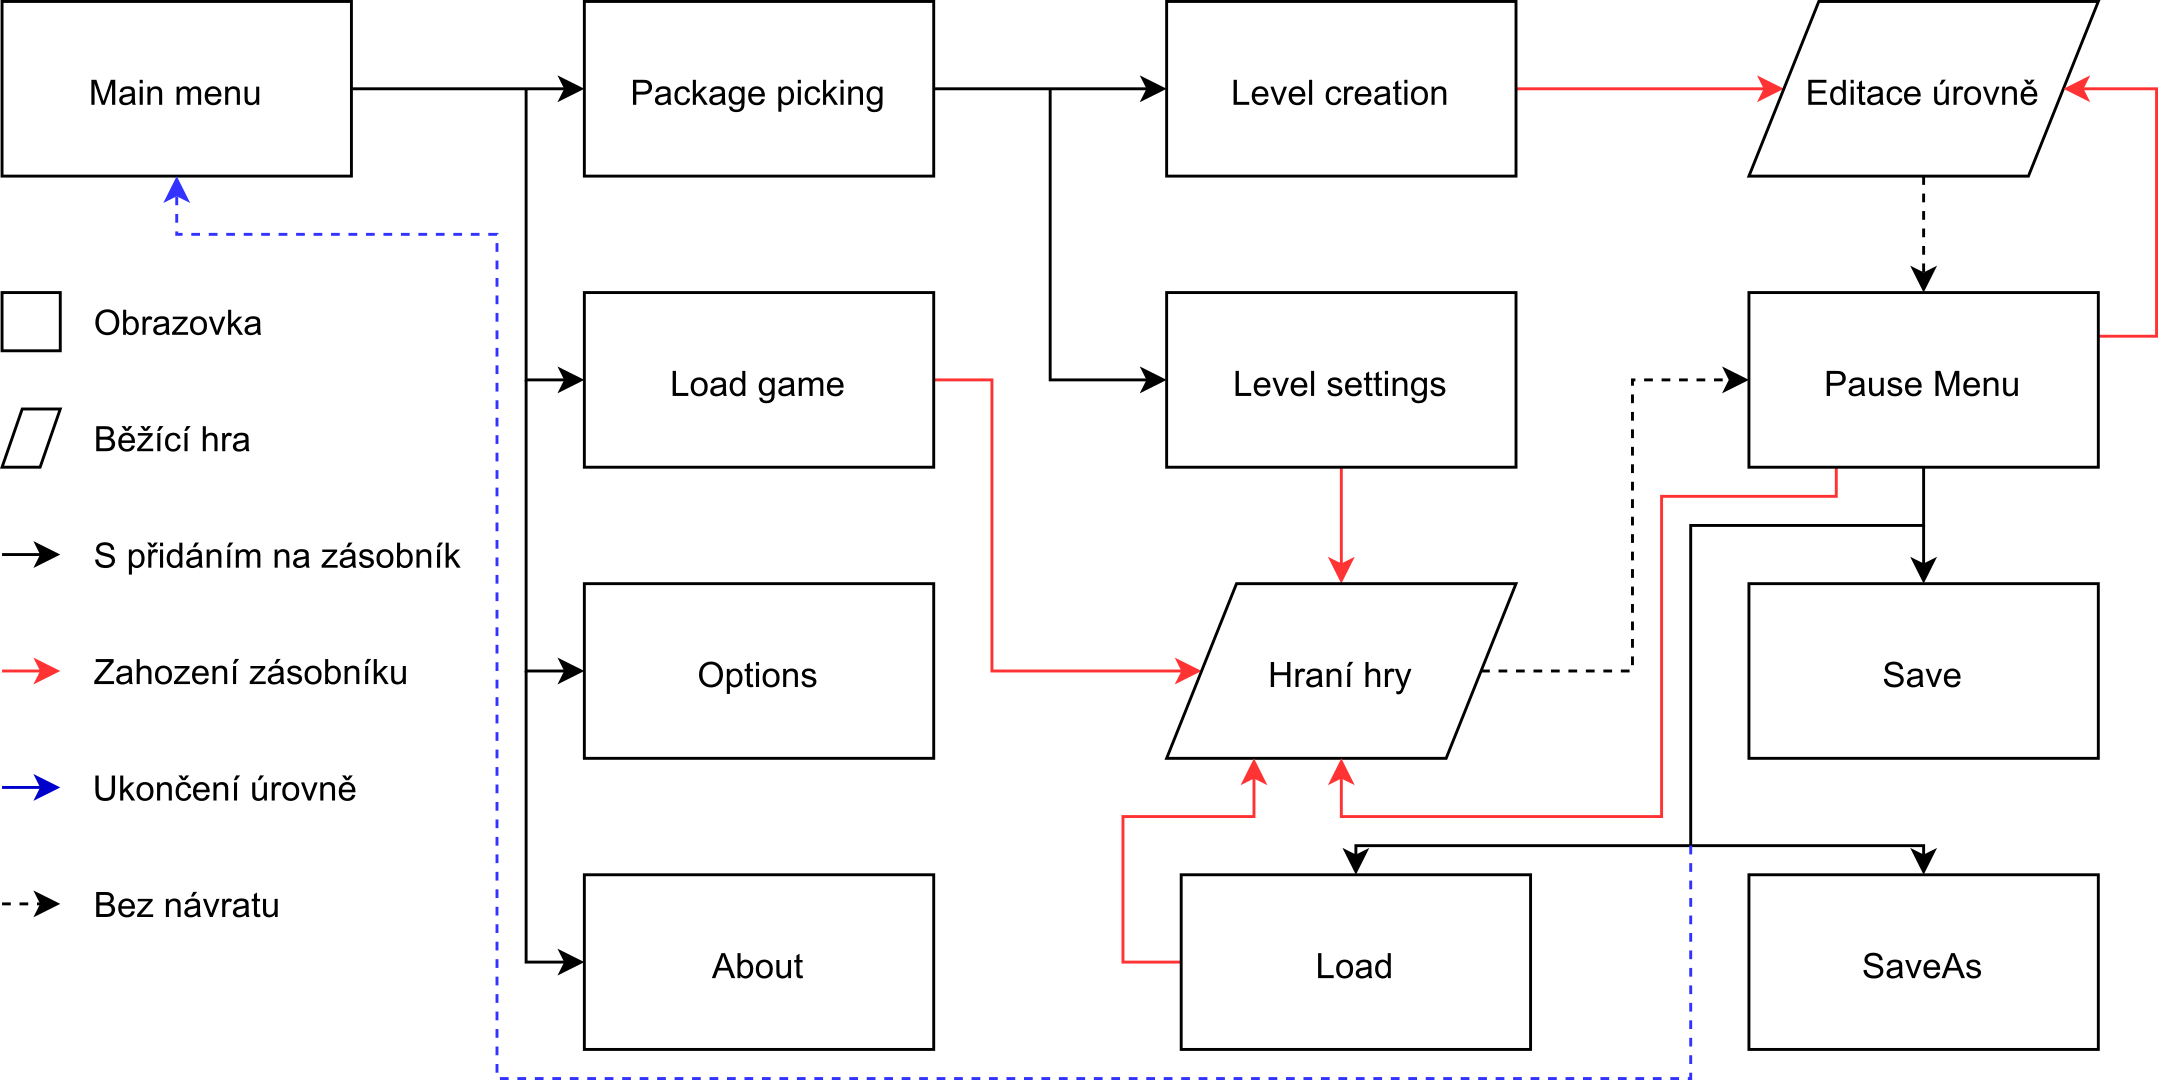
\includegraphics[width=\textwidth]{img/ScreenStructure.png}
	\caption{Obrazovky menu a přechody mezi nimi.}
	\label{fig:screen_structure}
\end{figure}


Vlastní akce přepnutí obrazovky je implementována vytvořením instance implementační třídy, která v rámci svého konstruktoru vytvoří danou obrazovku. Toto vytvoření probíhá za použití souborů definujících rozložení prvků, které jsou voláním \texttt{UI.LoadLayoutToElement} použity pro vytvoření objektové reprezentace uživatelského rozhraní uvnitř enginu. Tato objektová reprezentace je následně přístupná i z našeho kódu, a je použitá pro další modifikace, například v reakci na akci uživatele.

Herní data potřebná pro zobrazení některých obrazovek, například herní balíček při zobrazení výběru úrovní, jsou zpřístupněna jako veřejná \textit{property} proxy tříd. Při zavolání metody \texttt{Show} je kontrolována přítomnost a validita poskytnutých dat. Implementační třída při své alokaci dostává referenci na proxy třídu, čímž dostává přístup k poskytnutým herním datům a je schopna je použít pro zobrazení obrazovky.



\subsection{Automatizace uživatelského rozhraní}

Pro účely testování byl vytvořen systém pro automatické přepínání obrazovek bez zásahu uživatele. Tento systém je možné použít vytvořením XML souboru a specifikací parametrů příkazové řádky.

Jedním z těchto parametrů je \uv{-ui [d|s] xmlFilePath}, který z kombinace poskytnuté cesty a přepínačů \uv{d|s} vytvoří cestu, z které nahraje XML soubor. Tento soubor musí být validní vůči schématu \texttt{MenuActions.xsd}. Z tohoto souboru jsou  nahrány třídy specifikující akce pro jednotlivé obrazovky. Tyto třídy jsou potomkem \texttt{MenuScreenAction} a jsou vždy určeny pro konkrétní obrazovku. Implementace každé z obrazovek zná sobě příslušící třídu a umí v ní zakódovanou akci vykonat. Dále je vytvořena instance \texttt{ActionManager}, která slouží jako kontejner těchto nahraných tříd a řídí jejich předávání jednotlivým obrazovkám.

Diagram \ref{fig:uiautomationload} je zjednodušením diagramu \ref{fig:startup} a ukazuje části inicializace platformy, ve kterých je prováděn tento systém. Jak můžeme vidět, při startu aplikace bez parametrů příkazové řádky je tento systém úplně přeskočen. 

\begin{figure}[h]
	\centering
	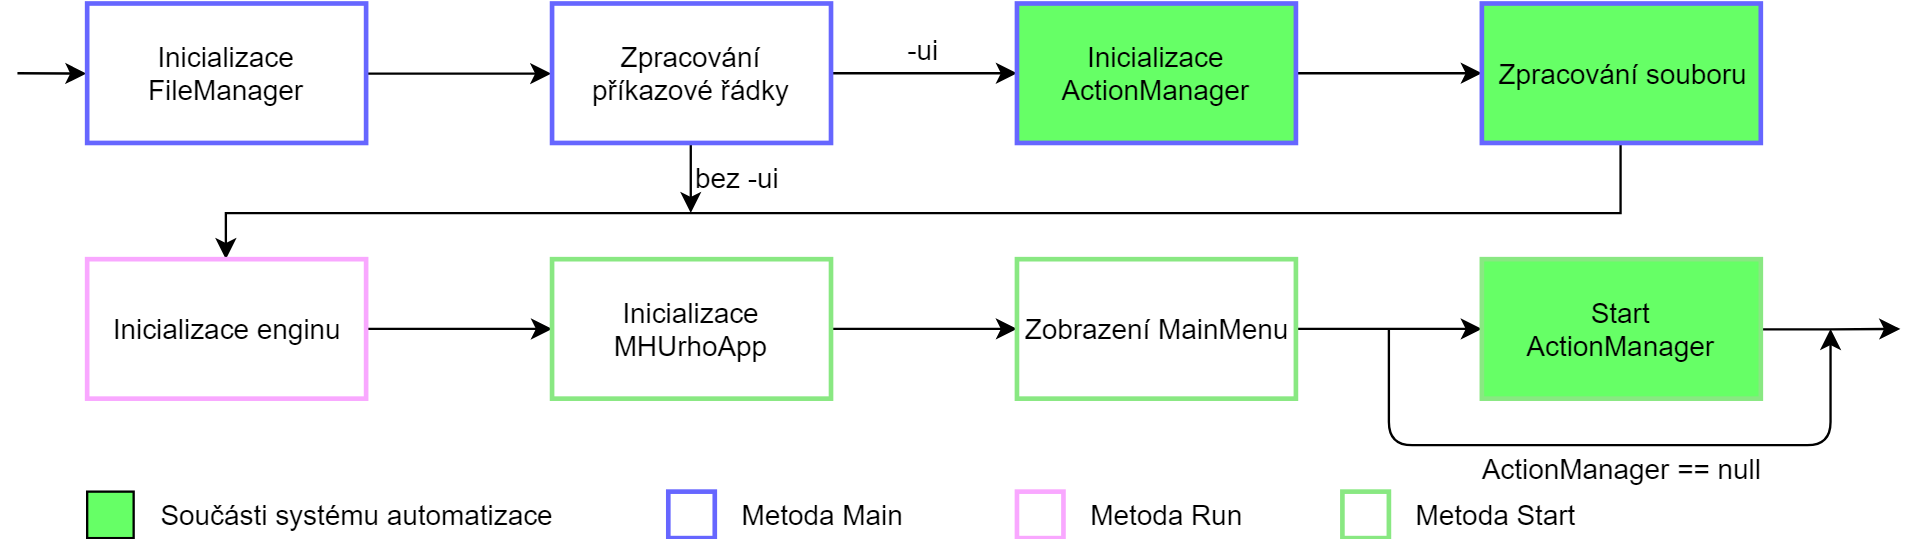
\includegraphics[width=\textwidth]{img/MenuActions.png}
	\caption{Nahrávání akcí v průběhu inicializace platformy.}
	\label{fig:uiautomationload}
\end{figure}



\section{Systém balíčků}
V části \ref{sec:packagestructure} jsme popsali základní strukturu systému balíčků. V této části popíšeme implementaci této struktury.

\subsection{Adresář balíčků}
\label{sec:packagedir}
Při instalaci hry je vytvořen adresář, ve kterém jsou uložena data generovaná aplikací či přidávaná uživatelem do aplikace. Tento adresář je v kódu označován jako \texttt{DynDataDir}, tedy adresář pro dynamická (měnící se) data. Jako součást tohoto adresáře je při instalaci vytvořen podadresář \texttt{Packages}, jehož účelem je centralizované umístění balíčků.

Obsah tohoto podadresáře můžeme vidět na diagramu \ref{fig:packagesdir}. Z pohledu platformy nejdůležitějším obsahem je soubor \texttt{Packages.xml}, ve kterém jsou uloženy záznamy o všech balíčcích dostupných ve hře. Tento soubor je ve formátu XML, splňujícího schéma \texttt{MHUrho.Desktop/Data/Schemas/GamePack.xsd}. Záznamy do tohoto souboru je možné přidávat v grafickém rozhraní při běhu platformy, konkrétně stisknutím tlačítka \texttt{Add} na obrazovce pro výběr balíčků \texttt{PackagePickingScreen}. Dále je možné při dodržení schématu editovat soubor manuálně a přidat tak balíčky mimo běh platformy. 

\begin{figure}[h]
	\centering
	\def\svgwidth{\textwidth}
	\input{img/DynData.pdf_tex}
	\caption{Typická struktura adresáře \texttt{DynDataDir}.}
	\label{fig:packagesdir}
\end{figure}

Tato struktura ukládání balíčků je vystavěna s myšlenkou uložení všech balíčků jako podadresářů adresáře \texttt{Packages}. Tato vlastnost ale není nijak vynucována či kontrolována, je tedy možné přidat i balíčky mimo tento adresář. Jedinou překážkou je nutnost použití relativní cesty vůči adresáři \texttt{Packages}.

\subsection{PackageManager}
\label{sec:packagemanager}
Třída \texttt{PackageManager} je základem celého systému balíčků. Jak můžeme vidět v části \ref{sec:init} na obrázku \ref{fig:startup}, vytvoření instance \texttt{PackageManager} je součástí inicializace platformy. První akcí na takto vytvořené instanci je načtení souboru \texttt{Packages.xml}, popsaného v předchozí části \ref{sec:packagedir}.

\begin{figure}[h]
	\centering
	\fontsize{8pt}{11pt}\selectfont
	\def\svgwidth{\textwidth}
	\input{img/PackageManager.pdf_tex}
	\caption{Datová struktura balíčků.}
	\label{fig:packagemanager}
\end{figure}

Na diagramu \ref{fig:packagemanager} můžeme vidět datovou strukturu systému balíčků. Při načtení souboru \texttt{Packages.xml}, případně při přidání balíčku do běžící hry, je pro každý balíček vytvořena jedna instance třídy \texttt{GamePackRep}, která je použita pro prezentaci tohoto balíčku uživateli při výběru pro načtení na obrazovce \texttt{PackagePickingScreen}. Instance třídy \texttt{GamePackRep} obsahuje pouze data potřebná pro její použití, tedy pro prezentaci balíčku a případné následné načtení balíčku. Těmito daty jsou:

\begin{itemize}
	\item jméno,
	\item popis,
	\item ikona,
	\item cesta k XML souboru.
\end{itemize}

Tato data jsou z XML souboru balíčku načtena při startu hry a zůstávají přítomna v paměti až do jejího ukončení. Zbylá data balíčku jsou načítána až po zvolení jednoho konkrétního balíčku hráčem. Ve hře je vždy nejvýše jeden načtený balíček, dostupný jako \texttt{ActivePackage} na třídě \texttt{PackageManager}.

Druhou funkcí třídy \texttt{PackageManager} je obalení rozhraní třídy \texttt{ResourceCache} poskytované enginem UrhoSharp. Tato třída umožňuje načítaní všech druhů assetů podporovaných enginem a jejich cachování. Bohužel přístup k této třídě je omezen na hlavní vlákno aplikace, tedy při přístupu z jiného vlákna, ve kterém implementujeme načítání hry, dochází k pádu aplikace. Pro zamezení chyb při programování načítání jsme vytvořili identické rozhraní na třídě \texttt{PackageManager}, které automaticky přesměrovává všechna volání na hlavní vlákno aplikace, kde následně zavolá odpovídající metodu \texttt{ResourceCache}.


\subsection{GamePack}
\label{sec:gamepack}


Třída \texttt{GamePack} představuje kompletně načtený balíček. Jak můžeme vidět na diagramu \ref{fig:packagemanager}, obsahuje tato třída referenci na instanci \texttt{GamePackRep} reprezentující daný balíček. Dále obsahuje tyto data:

\begin{itemize}
	\item typy dlaždic,
	\item typy jednotek,
	\item typy budov,
	\item typy projektilů,
	\item typy surovin,
	\item typy hráčů,
	\item typy logik úrovní,
	\item seznam úrovní,
	\item defaultní typ dlaždice,
	\item textury ikon.
\end{itemize}

Tato data jsou načítána podle jejich popisu v XML souboru, splňujícího schéma \texttt{MHUrho.Desktop/Data/Schemas/GamePack.xsd}. Soubor je vůči tomuto schématu validován jak při načítání reprezentanta balíčku (\texttt{GamePackRep}), tak při načítání celého balíčku. Pro zjednodušení manuální manipulace s tímto XML souborem jsme vytvořili třídu v souboru \texttt{GamePackXml.cs}, které tvoří objektovou reprezentaci tohoto schématu. Tedy pokud je v elementu \texttt{TileType} požadován potomek \texttt{texturePath}, pak singleton instance třídy \texttt{TileTypeXml} bude obsahovat položku \texttt{TexturePath}, kterou bude možno použít v metodě \texttt{XElement.Element()} jako argument pro získání tohoto potomka. Tímto způsobem je izolován zbytek kódu platformy od změn ve formátu či jménech elementů ve schématu. Další výhodou tohoto přístupu, a důvodem použití návrhového vzoru \textit{Singleton}, je reprezentace dědičnosti ve schématu pomocí dědičnosti v jeho objektové reprezentaci.

Při hře slouží tato třída jako databáze typů, tedy obsahuje metody pro získání reference na typy z výčtu výše podle jména či podle číselného identifikátoru. Jméno i identifikátor jsou načítány z XML souboru, ve kterém je jejich přítomnost vyžadována schématem.

Poslední funkcí je přístup k úrovním obsaženým v balíčku. Úrovně jsou, podobně jako balíčky samotné, před vlastním načtením reprezentovány separátní třídou \texttt{LevelRep}. Tato třída, podobně jako \texttt{GamePackRep}, obsahuje data potřebná pro výběr a nastavení úrovně před jejím spuštěním. Dále tato třída umožňuje manipulaci s úrovní z pohledu assetu, tedy její ukládání při editaci, vytvoření kopie pro editaci, načtení pro hru atd. Toto chování je implementováno podle návrhového vzoru \textit{State}.

\subsection{Assety}
Pojmem assety označujeme v naší práci veškerá data použitelná pro implementaci hry. Patří mezi ně například:

\begin{itemize}
	\item 3D modely,
	\item textury,
	\item XML data,
	\item části logiky poskytované enginem.
\end{itemize}

Každý typ entity, tedy budovy, jednotky či projektilu, má definovanou svou množinu assetů, které ji reprezentují při zobrazení či při výpočtu kolizí. Pro dodání assetů instancím těchto typů poskytujeme tři způsoby definice.

Prvním způsobem je explicitní specifikace assetů přímo v XML souboru balíčku. Tento způsob je implementován třídou \texttt{ItemsAssetContainer}, která z XML elementu vyčte všechna potřebná data a při požadavku vytvoří reprezentaci entity v herním enginu. Bližší popis reprezentace hry v herním enginu můžete nalézt v části \ref{sec:scenegraph}.

Druhým způsobem je využití funkcionality poskytované herním enginem a s ním distribuovaným editorem. V tomto editoru lze definovat reprezentaci entity a následně tuto definici serializovat do XML či binárního souboru, do takzvaného \textit{prefab}, neboli prefabrikátu. Pro tento způsob poskytujeme dvě třídy, \texttt{XmlPrefabAssetContainer} a \texttt{BinaryPrefabAssetContainer}, které obalí soubor definující reprezentaci entity a při instanciaci je použijou pro její vytvoření.

Použitý způsob je specifikován v XML popisu typu entity, a v závislosti na zvoleném způsobu jsou dále požadována další data, specifická pro daný způsob. Použití XML či Binary prefab umožňuje využití všech možností UrhoSharp enginu. Námi implementovaný \texttt{ItemsAssetContainer} umožňuje zjednodušenou specifikaci bez externích nástrojů, jakým je editor Urho3D, zato ale omezuje použitelné součásti enginu na tuto podmnožinu:

\begin{itemize}
	\item \texttt{Static model},
	\item \texttt{Animated model},
	\item \texttt{Collision shape},
	\item nastavení \texttt{Scale}.
\end{itemize}

Ke každému z modelů navíc umožňuje nahrát jeho textury. Tato podmnožina je podle nás dostatečná pro tvorbu graficky jednodušších her, proto schopnosti \texttt{ItemsAssetContainer} nijak rozšiřovat.

\subsection{Načítání balíčku}

Načítání balíčku je implementováno metodou Load, jejíž prototyp je:
\begin{lstlisting}
public static async Task<GamePack> Load(string pathToXml,
GamePackRep gamePackRep,
XmlSchemaSet schemas,
IProgressEventWatcher loadingProgress = null)
\end{lstlisting}

Už podle deklarace metody vidíme, že se implementace pokouší o asynchronní načítání balíčku. Nejedná se úplně o asynchronní načítání v pravém slova smyslu, protože drtivou většinu dat je nutno načítat na hlavním vlákně z důvodu restrikcí herního enginu, blíže popsaným v části \ref{sec:packagemanager}. Hlavním cílem je tedy rozdělit načítání na části, mezi kterými je platforma schopna nadále zpracovávat vstup od hráče. Tímto se snažíme zamezit tzv. \uv{zamrzání} aplikace, kdy aplikace z pohledu uživatele nic nedělá a odmítá reagovat na jakýkoli vstup od hráče. V prvních verzích bez tohoto přístupu jsme naráželi na problém, kdy systém Windows považoval náš proces za mrtvý a navrhoval nám jej zabít. Touto implementací jsme tomuto problému zabránili a navíc jsme umožnili notifikovat hráče o průběhu načítání.

Z pohledu implementace vlastního načítání je princip vcelku jednoduchý. Posloupnost akcí je následovná:

\begin{enumerate}
	\item načíst a validovat XML soubor;
	\item načíst typy dlaždic, jednotek, budov, projektilů, surovin;
	\item načíst typy logik hráčů a úrovní;
	\item načíst textury ikon;
	\item načíst reprezentanty úrovní,
	\item zavřít XML soubor.
\end{enumerate}

Při jakékoli chybě načítání, ať už nevalidnímu XML či chybějícímu souboru některého assetu, je načítání zastaveno, dosud načtená data znovu odalokována, chyba zalogována a zpět vypuštěna výjimka typu \texttt{PackageLoadingException}, signalizující chybu při načítání balíčku.

